%%%%%%%%%%%%%%%%%%%%%%%%%%%%%%%%%%%%%%%%%%%%%%%%%%%%%%%%%%%%%%%%%%%%%%%%%%%%%%%
% CONTRIBUTION TO THE SURFEX BOOK1: "Surface Processes Scheme"
% Author        : P. Tulet
% Original      : January 05, 2009
% Last Update   : January 05, 2009
%%%%%%%%%%%%%%%%%%%%%%%%%%%%%%%%%%%%%%%%%%%%%%%%%%%%%%%%%%%%%%%%%%%%%%%%%%%%%%%

\chapter{Chemistry and aerosols}
\minitoc
%=========================
\bibliographystyle{plain}
%=========================

\section{Dust aerosols}

Dust is mobilized from dry desert surfaces when the wind friction 
speed reaches a threshold wind friction speed of approximately
0.2 m/s. Dust is an important aerosol with annual global
 emissions ranging from 1000 to 3000 $Tg~yr^{-1}$ and average global
load around 10-30 $Tg$ (Zender \etal (2004)\nocite{Zender2004}).

Dust is mobilized by two related processes called saltation and 
sandblasting. Saltation is the horizonal movement of soil grains in a turbulent
near surface layer. Sandblasting is the release of fine dust when 
the saltating grains hit the surface. Several papers document these two
processes. (Marticorena and Bergametti (1995)\nocite{Marticorena1995} and references therein describe the physics
of saltations, and Shao \etal (1993)\nocite{Shao1993} describe the physics of sandblasting.


\subsection{Implementation in the Externalized surface}

The dust fluxes are calculated using the Dust Entrainment And Deposition
(DEAD) model (Zender \etal (2003)\nocite{Zender2003}). This model is based on Marticorena and Bergametti (1995).
The dust fluxes are calculated consistently with the ISBA soil surface
scheme. Table \ref{tbl:input} gives an overview of the main input to the dust 
production model.


\begin{table*}[htb]
\caption{ISBA variables used by the dust module \label{tbl:input}}
\begin{tabular}{|c|c|c|}
\hline
PARAMETER            &  EFFECT ON DUST EMISSION  & REFERENCE    \\
\hline
\hline
wind friction speed  & Increase emissions          & Marticorena and Bergametti (1995) \\
\hline
Soil moisture        & Inhibit emissions           & Fecan \etal (1999)\nocite{Fecan1999}       \\
\hline
Vegetation fraction  & Inhibit emissions           & Marticorena and Bergametti (1995)\\
\hline
Surface roughness    & Inhibit emissions           & Laurent \etal (2005)\nocite{Laurent2005} \\
\hline
Surface texture      & Soil sizes $ > ~50 {\mu}m$  &                       \\
                     &  increase saltation flux    & Iversen and White (1982)\nocite{Iversen1982}        \\
\hline 
\end{tabular}
\end{table*}


\subsection{Features of the model}

%plm=======================================================================================
\subsubsection{Emission process}
The production of desert aerosols follows in fact the sandblasting process
following the bombing of the aggregates present at the surface by particles in saltation
(Figure \ref{fig_chap5_1}). These processes depend on both weather conditions and surface states.
 Indeed, the kinetic energy of the grains caused by saltation is used in
shocks induced by these particles, when they fall to the ground to release and eject fine
particles constituting aggregates (Gillette and Goodwin (1974)\nocite{Gillette1974}, Gomes \etal (1990)\nocite{Gomes1990}). The
resistance to wrenching, concerns soil properties like the gravity force and the
inter-particle forces.
Moreover, emission of aerosols is a threshold phenomenon: it occurs only when the wind
friction force exerted on soil grains becomes greater than the forces that
maintain them to the ground. When this threshold is exceeded, the soil grains start
moving horizontally. The smallest particles can be suspended
in the atmosphere and constitute the desert aerosol.
The production intensity of fine particles thus depends on the ratio between the transfered kinetic energy
flow and the cohesion forces of the particles forming the aggregates.

\begin{figure}[h]
\begin{center}
\psfig{figure=\EPSDIR/fig_chap5_1.pdf,width=10cm}
\caption{illustration of the two main processes involved in the emission of aerosols desert (saltation and sandblasting) when the
erosion threshold is exceeded. \label{fig_chap5_1}}
\end{center}
\end{figure}

Once the particle is injected into the atmosphere, the forces to which it is subjected will
control its suspension. It is generally accepted, given the balance of forces, that only
particles with a diameter less than about 20 \textmu m can be transported (Nickling (1994)\nocite{Nickling1974}). 
Those fine particles, named aerosols, constitute the main part of the vertical flow of
desert aerosol ($F$). This vertical flow is defined as the mass of particles crossing per unit of time
a unitary surface parallel to the surface.

\subsubsection{Parameterization of the friction velocity}
Wind is the driving force in the aerosols desert generating process. The
ground surface opposes the air flow and slows the air mass at its base. The surface wind
is very sensitive to changes in surface characteristics at small
scale. These changes may be due, for example, to the presence of vegetation or
rocks. In the first few meters of the atmosphere, a surface boundary layer (CLS)
develops, in which the horizontal component of the wind speed has a
vertical gradient whose intensity depends on the ability of the soil surface to slow the
flow (Figure \ref{fig_chap5_2}). For a laminar flow over a horizontal surface, the
shear constraint ($\tau$) exerted by the wind on the surface is connected to the vertical gradient
of the wind speed ($U$) by:

%eq1
\begin{equation}
\tau = \mu~~\frac{\partial U}{\partial Z}
\end{equation}
	
Where $\mu$ is the air dynamic viscosity coefficient and Z the height above the ground.

\begin{figure}[h]
\begin{center}
\psfig{figure=\EPSDIR/fig_chap5_2.pdf,width=10cm}
\caption{Representation of the effect of soil on the airflow and of the shear stress $\tau$ 
exerted by the flow on the ground. \label{fig_chap5_2}}
\end{center}
\end{figure}


The shear constraint can also be expressed in terms of friction wind speed
$U_*$, which is usually the physical quantity used to quantify
friction forces exerted by wind on a surface:

%eq2
\begin{equation}
\tau = \rho_{a}~U_{*}
\end{equation}


Where $\rho_{a}$ is the air density.
Under conditions of thermal neutrality, $U_*$ can be determined from the wind speed
$U$ at a height $z$ from the ground and the height of aerodynamic roughness ($Z_0$) using a
wind speed logarithmic profile (Priestley (1959)\nocite{Priestley1959}:

%eq3
\begin{equation}
U(Z) = \frac{U_*}{\kappa}\ln(\frac{z}{Z_0})
\end{equation}


Where $\kappa=0.4$ is the Von Karman constant. \\
Physically, $Z_0$ reflects the length scale of the sink of air momentum
induced by the surface roughness. More specifically, $Z_0$ represents quantitatively the effect
of erodible elements (soil grains) or non-erodible ones (rocks or vegetation) on the transfer
of wind energy to the surface.

\subsubsection{Friction velocity threshold }

The resistance of the surface on the motion is represented by the 
friction velocity threshold $U_{*_t}$. Indeed, the friction velocity threshold $U_{*t}$ controls both the frequency and
the intensity of emissions of aerosols desert, so it is important to parameterize carefully
$U_{*_t}$ and give special attention to obtain the quantities it depends on.
The erosion threshold is mainly computed from the soil grains diameter $D_p$, the surface roughness
($Rug$) and the soil moisture ($w$).
The friction velocity threshold is expressed as:

%eq4
\begin{equation}
U_{*_t} = U_{*_t}(D_p) \cdot F(Rug) \cdot F(w)
\end{equation}


	
$U_{*_t}(D_p)$: depends on the friction speed with the diameter of soil grains.
$F(Rug)$ and $F(w)$: weighting functions of the influence of roughness and soil moisture.
Under idealized conditions, ie for a smooth surface and a loose and dry soil, the
friction velocity threshold $U_{*_t}(D_p)$ can be determined using the formulation of
Marticorena and Bergametti (1995), which consists in adjusting an empirical expression
as a function of the particle diameter. Under standard atmospheric conditions
($\rho_a = 0.00123 g \cdot cm^{-3}$, $\rho_p = 2.65 g \cdot cm^{-3}$), the friction velocity threshold $U_{*_t}(D_p)$ is
given by:

%eq5
%U_{*_{t}}(D_p) = \left [ \frac{0.1666681\rho_{p} g D}{-1+1.928 {Re_{*_t}}^{0.0922}} \left ( 1+ \frac{6\times 10^{-7}}{\rho_{p} g D^{2.5}} \right ) \right ] ^{1/2} \rho ^{-1/2} \hspace{1cm}, 0.03\leq Re_{*_t} \leq 10 \\
\begin{eqnarray}
U_{*_{t}}(D_p) = \frac{0.129 K}{ { \left ( 1.928 {Re_{*_t}}^{0.092} \right ) }^{0.5}} \hspace{1cm}, 0.03\leq Re_{*_t} \leq 10 \\
U_{*_{t}}(D_p) = 0.129  K \left [ 1-0.0858 \exp \left ( -0.0617 \left ( Re_{*_t}-10 \right ) \right ) \right ] \hspace{0.1cm}, {Re_{*_t}} > 10 
\end{eqnarray}

Where $Re_{*_t} = U_{*_t} D_p / \nu$ is the Reynolds number threshold ($\nu = 0.157~cm^{2}s^{-1}$: kinematic viscosity) \\ \\
and: $K = \left ( \frac{\rho_{p} g D_p}{\rho_{a}} \right ) ^{0.5} \left ( 1+\frac{0.006}{\rho_{p} g {D_p}^{2.5}} \right ) ^{0.5}$ \\ \\
%The friction velocity threshold is calculated in the code by the routine "wnd_frc_thr_slt_get which
%is in the module mode_dstmblutl.F90. 
The optimal diameter of the particle is equal to 75 \textmu m.

\subsubsection{Influence of soil moisture on friction velocity threshold}

The presence of interstitial water between soil grains has the effect of increasing the
cohesion of the soil, thus increasing the friction velocity threshold. This increase is
integrated in the module DEAD from the parameterization developed by Fecan \etal (1999). 
The proposed equation, expresses the threshlod increase, under wet conditions $U_{*_{tw}}$
compared to that in dry conditions.

%eq7 et eq8

\begin{eqnarray}
U_{*_{tw}} = U_{*_{t}} ~~~~~~~~~~ for~ w ~ < ~ w^{'} \\
U_{*_{tw}} = U_{*_{t}} {\left [ 1+1.21(w-w^{'})^{0.68} \right ]} ^{0.5} ~~ for~ w ~ > ~ w^{'}
\end{eqnarray}



With:
$w$: mass soil moisture (\% mass water / mass dry soil).
And soil moisture threshold is given by: 

%eq9
\begin{equation}
w^{'} = 0.17 (\%clay) + 0.14 (\%clay)^{2}
\end{equation}

%The effect of soil moisture on friction velocity threshold is treated by the
%routine "frc_thr_ncr_wtr_get" in module "mode_dstmblutl.F90.

\subsubsection{Aerodynamical roughness height}

The effects of the internal boundary layer (IBL) on friction velocity threshold, due to the presence of stones,
is set in DEAD scheme by Marticorena and Bergametti (1995). The energy distribution is defined in this parameterization as the
ratio between the IBL shear friction and the total shear friction of the surface boundary layer (SBL). This ration is given by:

%eq10
\begin{equation}
f_{eff}(Z_0,Z_{0s}) = 1 - \left [ \ln(Z_0/Z_{0s}) / \ln(0.35(10/Z_{0s})^{0.8}) \right ]
\end{equation}

	
$Z_{0s} = 33.3 \times 10^{-6}~m$: roughness length of the smooth surface \\
$Z_0 = 100.0 \times 10^{-6}~m$: roughness length of the erodible surface\\
The friction velocity threshold is expressed as:

%eq11
\begin{equation}
U_{*_t}(D_p,Z_0,Z_{0s}) = \frac{U_{*_t}(D_p)}{f_{eff}(Z_0,Z_{0s})}
\end{equation}

%This ratio is calculated by the routine "frc_thr_ncr_drg_get" in the module
%"Mode_dstmblutl.F90.

\subsubsection{Surface flux}

The horizontal saltation flux ($G$) is calculated in module DEAD through the
White (1979)\nocite{White1979} relationship :

%eq12
\begin{equation}
G = c \cdot \frac{\rho}{g}{U_*}^{3} \left ( 1-\frac{U_{*_t}}{U_{*}} \right ) \left (  1+\frac{U_{*_t}}{U_{*}} \right )
\end{equation}

With $c=2.61$. The ratio between the vertical flux and the horizontal flux is a function of clay content.
For contents between 0 and 20\%, this ratio is :

%eq13
\begin{equation}
\alpha = \frac{F}{G} = 100 \exp { \left [  ( 13.4 (\%clay) - 6 ) \times \ln(10) ~\right ] }
\end{equation}

	
In the DEAD  module, the fraction of clay is considered constant and is equal to 20\%.
The final vertical flux is averaged by a pre-determined factor equals to 0.0021 and by the sand fraction.

%plm=======================================================================================

\subsubsection{Mass flux repartition}
Upon Alfaro and Gomes (2001)\nocite{Alfaro2001} the mass flux is partitioning on the different modes upon  the surface friction velocity. More the
collision energy is strong more the dust aggregates can be separates into small particles.
In surfex, two possibilities are offered. Users can fix the partitioning or the mass flux on the differents modes considered, or compute automatically this partitioning upon the ISBA friction velocity.
In this latter case, Alfaro and Gomes (2001)\nocite{Alfaro2001} gives the following partitionning:
\begin{itemize}
\item u* less than 0.32 $m.s^{-1}$, all particles are emitted in the coarse mode.
\item u* at 0.42 $m.s^{-1}$,  63 \% of the mass flux is in the bigger coarse mode (D=14.2 $\mu m$) ,  36 \% in the lower coarse mode (D=6.7 $\mu m$), and 1 \% in the accumulation mode (D=1.5 $\mu$ m)
\item u* at 0.50 $m.s^{-1}$,  49 \% of the mass flux is in the bigger coarse mode (D=14.2 $\mu m$) ,  43 \% in the lower coarse mode (D=6.7 $\mu m$), and 8 \% in the accumulation mode (D=1.5 $\mu$ m)
\item u* at 0.66 $m.s^{-1}$,  9 \% of the mass flux is in the bigger coarse mode (D=14.2 $\mu m$) ,  76 \% in the lower coarse mode (D=6.7 $\mu m$), and 15 \% in the accumulation mode (D=1.5 $\mu$ m)
\end{itemize}
Between these friction velocities values, the mass flux partitioning is linearly interpolated.

\section{Sea Salt emission}
Sea salt aerosols are produced as film and jet droplets when bubbles, entrained in the water by breaking waves, disrupt the sea surface (Blanchard, 1983), and at winds speeds exceeding about 9 $m.s^{-1}$, by direct disruption of the wave tops (spume droplets) (Monahan \etal (1983)\nocite{Monahan1983}).

Sea Salt emission are parameterized upon the  formulation of Vignati \etal (2001)\nocite{Vignati2001} (effective source function) or upon a lookup table defined by Schulz \etal (2004)\nocite{Schulz2004}.
Vignati \etal (2001) gives a formulation of particles emission upon the wind at 10 meters as:
\begin{itemize}
\item $F(R=0.2 \mu m) = 10^{0.09 U_{10m} + 0.283} particles.cm^{-2}.s^{-1}$ 
\item $F(R= 2 \mu m) = 10^{0.0422 U_{10m} + 0.288} particles.cm^{-2}.s^{-1}$
\item $F(R= 12 \mu m) = 10^{0.069 U_{10m} - 3.5} particles.cm^{-2}.s^{-1}$
\end{itemize}

\section{Dry deposition of gaseous species}

The removal of gases from the atmosphere by turbulent transfer and uptake at
the surface is defined as dry deposition. This process enables some
chemically reactive gases to be efficiently removed from the atmosphere. 
Dry deposition is usually parametrized through a deposition velocity $v_d$,
defined by $v_d=-\frac{F_c}{c(z)}$, where $F_c$ is the flux of the considered
compound ($F_c$ is assumed constant over the considered range of heights) and
$c(z)$ is the concentration at height $z$ (molecules/cm$^3$). $v_d$ depends
on many variables such as wind speed, temperature, radiation, the considered
species and the surface conditions. It is commonly described
through a resistance analogy often called "Big-Leaf" Model 
(e.g.  Wesely and Hicks (1977)\nocite{Wesely1977}).
\[
v_d(z)=\frac{1}{R_a+R_b+R_c}\]
where $R_a$ is the aerodynamic resistance, which is a function of the
turbulence 
in the boundary layer, $R_b$ the quasi-laminar resistance partially controlled
by molecular diffusion, and $R_c$ the surface
resistance, which combines all the transfer pathways playing a role in the
uptake of trace gases by the surface.

\begin{figure}[htb]
\centerline{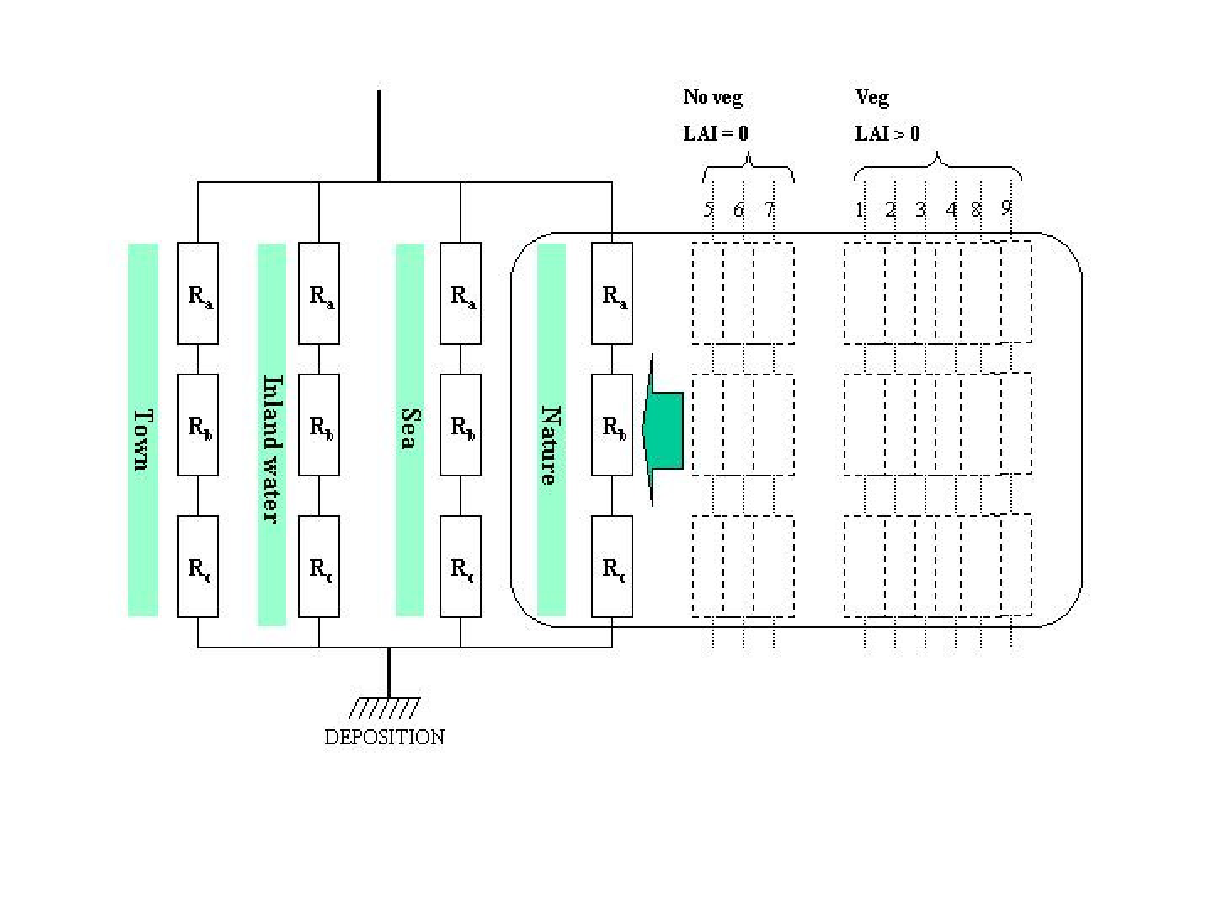
\psfig{file=\EPSDIR/schema_dep.pdf,width=0.9\textwidth}}
\caption{\sl ~{Schematic resistances for dry deposition module in
accordance with the surface state. 
Ra represents the aerodynamic resistance, Rb the quasi-laminar
resistance and Rc the surface resistance.}}
\label{schema} 
\end{figure}

\subsubsection*{Meso-NH surface for dry deposition}
As shown fig. \ref{schema}, earth surface is divided into four major
parts. On those surfaces calculation of specific parameters are done
(friction velocities, surface resistances, ...). The earth splitting
is done as follows : town horizontal fraction Masson (2000)\nocite{Masson2000}, inland
water and sea surfaces (differents because of their surface
temperature) and nature fractions. Nature surface is cut into 9 cover type, 
which can be reorganized by 'patches' (1 to 9). 
One 'patch' contains one or several cover types (user choice). 
These cover types are connected with the Wesely classes of
vegetation for the surface resistance data parameters (see table
\ref{classveg}).
\begin{table}
\begin{center}
\begin{tabular}{|l|l|} \hline
\bf{Meso-NH nature cover type} & \bf{Wesely correspondence class} \\ \hline 
 C3 cultures types(low) &       (2) Agricultural land \\ 
 C4 cultures types(hight)&      (2) Agricultural land \\ 
 forest and trees       &       (4) Deciduous and (5) coniferous
 forest \\ 
 grassland              &       (3) Range land \\ 
 no vegetation (smooth) &       (8) Baren land, mostly desert \\  
 no vegetation (rocks)  &       (11) Rocky open areas with low-growing
 shrubs \\ 
 permanent snow and ice &        No correspondence \\ 
 irrigated crops        &       (9) None forested wetland \\ 
 irrigated parks gardens or peat bogs   & (6) Mixed forest including
 weet land\\
                        &                  and (9) none forest wetland \\ 
\hline
\end{tabular}
\caption{\sl ~{Meso-NH vegetative cover type and Wesely connected
class for dry deposition calculation}}
\label{classveg}
\end{center}
\end{table}

%&&&&&&&&&&&&&&-------------GG0------------------

\subsection{Resistances for dry deposition}
\subsubsection*{Aerodynamic resistance $R_a$}

$R_a$ determines the rate of transport of gases between a given level in the
atmosphere and the height of the effective surface sink. 
It is usually calculated as the bulk aerodynamic resistance to the transfer of
momentum :  $R_a(z_R)=\frac{1}{\bf{C_D} \bf{V_A}}$, where $\bf{C_D}$ is the drag
coefficient for momentum (see for example Wesely and Hicks (1977); Sheih \etal (1979)\nocite{Sheih1979};
Walcek \etal (1996)\nocite{Walcek1996})
and $\bf{V_A}$ the wind speed (in the following, the parameters which are
already used or calculated in the MESO-NH subroutines will be noted in bold
characters).
%-------------------------GG1
% The $\bf{C_D}$ coefficient is calculated in the ISBA scheme.
%-------------------------GG1
The reference height $z_R$ is taken as the lowest atmospheric level in
the ISBA scheme.
\medskip

An alternate way is to use the ISBA calculation of $\bf {R_a}$,
$\bf{R_a(z_R)}=\frac{1}{\bf{C_H} \bf{V_A}}$ 
which determines the transfer of water
vapor. $\bf{C_H}$ is then the drag coefficient depending upon the thermal
stability of the atmosphere.  \\
%--------------------------GG2
Heat drag coefficients are calculated in WATER\_FLUX for inland water
and sea, in URBAN for artificial land (town) and in ISBA for the other 
nature cover types or patch. So there is one $\bf {R_a}$ different for
each different coefficient.
\\
This formulation of $\bf {R_a}$ requires an additional term to the
quasi-laminar resistance described below.
%--------------------------GG2
\subsubsection*{Quasi-laminar resistance $R_b$}

The component $R_b$ is associated with transfer through the quasi-laminar 
layer in contact with the surface. $R_b$ quantifies the way in which pollutant
or heat transfer differ from momentum transfer in the immediate vicinity of the
surface (this is due to the effects of molecular diffusion and the difference 
of roughness lengths found for momentum and mass transfer). 
$R_b$ depends on both turbulence characteristics and the molecular
diffusion of the considered gas. Transport of a gas through the
quasi-laminar layer by molecular diffusion depends on the thickness of the
layer, the concentration gradient over the layer and on a diffusion constant,
which in turn depends on the radius of the gas molecule and on the temperature.
The complexity of vegetation generally limits the accuracy with which the
magnitude of this mechanism can be estimated in the field. This resistance can
be conveniently written as:
\[ R_b=\frac{1}{k u^*} \log (\frac{z_0}{z_c})\]
$k$ is the Von Karman constant and $u^*$ the friction velocity.
$z_c$ is the roughness length for the pollutant under investigation (Baldocchi et al. (1987)). 

According to Hicks \etal (1987)\nocite{Hicks1987}, Garrat and Hicks (1973)\nocite{Garrat1973}
$R_b$ can be approximated for vegetation and fibrous roughness elements by :
\[ R_b = \frac{2}{\bf{k} \bf{u^*}}(\frac{Sc}{Pr})^{2/3} \]
$Sc$ and $Pr$ are the Schmidt and Prandtl numbers respectively.
$Pr=0.72$ and $Sc=\frac{\nu}{D_i}$, with $\nu$ the kinematic viscosity of
air (0.15 cm$^2$s$^{-1}$, 20$^o$ C, p = 1 atm) and $D_i$ the molecular
diffusivity of gas $i$ (see table \ref{const} for some of these
constants). 
%----------------GG3------------------
For snow, ice, water and bare soil, $R_b$ can be calculated by (Ganzeveld and Lelieveld (1995)\nocite{Ganzeveld1995}):\[ R_b =
\frac{1}{\bf{k} \bf{u^*}}(\frac{Sc}{Pr})^{2/3} \]\\
This formulation is used for all Meso-NH grid fraction cover with no
vegetation (Leaf Area Index = 0), that include artificial land, water
and sea.\\
Definition of friction velocity in MNH is given by : $u^* =
\sqrt[4]{{\bf {<u'w'>}_{xx}}^2+{\bf{<v'w'>}_{xx}}^2}$. Where $<u'w'>_{xx}$ and
$<v'w'>_{xx}$ represents   
surface fluxes of horizontal momentum in x and y directions (xx for sea,
water, town and nature patch).
%----------------GG3------------------
Molecular diffusivity species/air  can be obtain by the knowledge of $H_2O/air$ diffusivity.
The coefficient of diffusivity is given by the general formula as:\\
$D = v l /3 = \frac{0.376 k T}{N (M Cste)^{0.5}}$\\
with
l mean free path,
v mean molecular velocity,
k Boltzmann constant,
T temperature,
N concentration,
M molecular mass.
So we use for computing molecular diffusivity: \\ 
$$
D(gaz)=D(H_2O) \left(\frac{M(H_2O)}{M(gaz)} \right)^{0.5}
$$
with 
$$
D(H_2O)= 2.22e-5 + 1.25 10^{-7} (T + 273)  for 193 K < T < 0 K
$$
$$
D(H_2O)= 2.22e-5 + 1.46 10^{-7} (T + 273)  for 273 K < T < 323 K 
$$

\medskip

However, these formulations of $R_b$ remain still controversial. 
Recent results from fields studies 
indicate that they
are not in agreement with experimentally derived results, at least
for the transfer of HNO$_3$
over wheat (Muller \etal (1993)\nocite{Muller1993}).
%-----------GG4--------------------
At last, velocity dry deposition is not very sensitive of the choosen
definition of $R_b$ (Ganzeveld and Lelieveld (1995)).
%-----------GG4--------------------
\subsubsection*{Surface Resistance $R_c$}

The surface resistance is the most difficult of the three resistances to
describe. $R_c$ values can be obtained from theoretical considerations based
for instance on solubility and equilibrium; calculations in combination with
simulation of vegetation specific processes, such as accumulation, transfer
process through stomata, mesophyll, cuticles, etc $\ldots$
(Baldocchi \etal (1987)\nocite{Baldocchi1987}, Wesely (1989)\nocite{Wesely1989}). The values of $R_c$ are based on
measurements of $V_d$. By determining $R_a$ and $R_b$ from the meteorological
measurements, $R_c$ is calculated as the residual resistance. The calculated
$R_c$ are then related to surface conditions, time of day, etc $\ldots$ in
order to obtain parametrizations of $R_c$.

\begin{figure}[htb]
\centerline{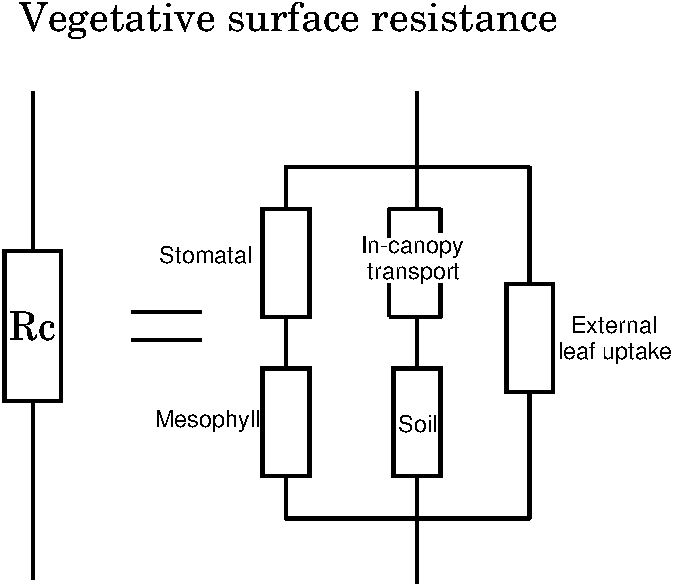
\psfig{file=\EPSDIR/surf.pdf,width=0.4\textwidth}}
\caption{\sl ~{Surface resistance schematic for vegetation.}}
\label{schema2}
\end{figure}
%-------------GG5-------------------------------
$R_c$ is a function of the canopy stomatal resistance $R_{stom}$ and mesophyll
resistance $R_m$, the canopy cuticle or external leaf resistance $R_{ext}$, the
soil resistance $R_{soil}$ and in-canopy resistance $R_{inc}$, 
and the resistance
to surface waters or moorland pools, $R_{wat}$, $R_{sea}$ (Erisman and Baldocchi (1994)\nocite{Erisman1994}).
In turn, these resistances are affected by leaf area index, stomatal
physiology, soil and external leaf surface, pH presence and chemistry of
liquid drops and films.
In summary, $R_c$ should be calculated as Erisman and Baldocchi (1994) :
\begin{itemize}
%\item {Vegetative surfaces :
%\[R_c={\left(\frac{1}{R_{stom}+R_m}+\frac{1}{R_{inc}+R_{soil}} +
%\frac{1}{R_{ext}} \rigth) }^{-1} \]}  
%\item {Water surfaces : \[R_c=R_{wat}\]}
%\item {Sea surfaces : \[R_c=R_{sea}\]}
%\item {Bare soil (no vegetation) : \[R_c=R_{no}\]}
%\item {Rock surfaces : \[R_c=R_{rock}\]}
%\item {Snow/ice  cover : \[R_c=R_{snow}\]}
%\item {Artificial land : \[R_c=R_{town}\]}
\item Vegetative surfaces :
$
R_c= \left(\frac{1}{R_{stom}+R_m}+\frac{1}{R_{inc}+R_{soil}} + \frac{1}{R_{ext}} \right)^{-1} 
$
\item Water surfaces : $R_c=R_{wat}$
\item Sea surfaces : $R_c=R_{sea}$ 
\item Bare soil (no vegetation) : $R_c=R_{no}$
\item Rock surfaces : $R_c=R_{rock}$
\item Snow/ice  cover : $R_c=R_{snow}$
\item Artificial land : $R_c=R_{town}$

\end{itemize}
%-------------GG5-------------------------------
\subsubsection*{Stomatal and mesophyll resistance $R_{stom}$ and $R_m$}

The stomatal resistance for water vapor is calculated in the ISBA subroutines
as \[ \bf{R_{stom}}=\frac{R_{smin}}{F_1 F_2 F_3 F_4\, LAI},\] where
$\bf{LAI}$ is the leaf area index computed by patch, and $F_1$, $F_2$,
$F_3$, $F_4$ are limiting factors depending on 
radiation, wetness of soil and temperature. In order to describe the stomatal
resistance for another gas, the ISBA $\bf{R_{stom}}$ for water vapor should be
corrected as followed :
\[ R_{stom,x}={\bf{R_{stom}}} \times \frac{D_{H_2O}}{D_x},\]
$D_{H_2O}$ and ${D_x}$ are the diffusion coefficients of $H_2O$ and $x$
respectively (Wesely (1989)).

\medskip

There is not much knowledge on the mesophyll resistance for different gases and
the conditions which determine its value. For some gases, such as SO$_2$ %3.e-2
O$_3$ %1.e-2
and NH$_3$, %1.5e-1
$R_m$ is experimentally found near zero values (Erisman and Baldocchi (1994)).
This is in agreement with the parametrization suggested by Wesely (1989)
for the calculation of the mesophyll resistance :
\[ R_{mx} = ( \frac{H^*}{3000} + 100 f_0) ^{-1} \] 
In this expression, $H^*$ is the Henry's law constant for the considered gas,
$f_0$ a reactivity factor which determines the rate of reduction of the
substance. Two parallel pathways are thus assumed, one for highly reactive
gases, the other one for soluble substances. Table \ref{const} 
lists $H^*$ and
$f_0$ for some species (Baer and Nester (1992)).

\begin{table}
\begin{center}
\begin{tabular}{lll} \hline
Species         & Reactivity factor     & Henry's law (M/atm) \\ \hline 
Sulfur dioxide  & 0     & $1.6(1+2.1\; 10^{-2}/H+)$ \\
Nitric oxide    & 0     & $1.9\; 10^{-3}$        \\
Nitrogen dioxide & 0.1  & $10^{-2}$              \\
Nitric acid      & 0    & $5.8\; 10^{6}/H+$       \\
Ozone           & 1.    & $1.5\; 10^{-2}$         \\
Hydrogen peroxide  & 0  & $1.8\; 10^{5}$          \\
Formaldehyde    & 0     & $3.26\; 10^{-4}$ \\
Aldehydes       & 0     & $76$ \\
Organic acids   & 0     & $1.45\; 10^{-4}$ \\
Organic peroxide  & 0.25& $665$ \\
Peroxyacetic acid  & 0.5& $1635$ \\
Peroxyacetyl nitrate &0.1& $3.6$ \\
Other alkanes & 0       & $1.\; 10^{-3}$ \\
Ethane           & 0    & $1.9\; 10^{-3}$ \\
Ethene           & 0    & $4.9\; 10^{-3}$ \\
Propene           & 0   & $4.7\; 10^{-3}$ \\
Butene and other olefins  & 0   & $1.3\; 10^{-3}$ \\
Toluene       & 0       & $0.15$ \\
Xylene      & 0         & $0.1$ \\ 
\hline
\end{tabular}
\caption{\sl ~{Reactivity factor and Henry's law constants for different chemical species}}
\label{const}

\end{center}
\end{table}

\subsubsection*{External leaf uptake $R_{ext}$}

The external leaf uptake can act as an effective sink, especially for soluble
gases at wet surfaces. 
%----------------GG6---------------------
The resistance of the outer surfaces in the upper canopy (leaf cuticular
resistance in healthy vegetation) is computed by Wesely (1989), for a
dry surface to any gas (x), as :
\[R_{ext.x.dry}=R_{ext}(10^{-5}H^*+f_0)^{-1}\]
In this expression, $R_{ext}$ is given by land category and season in table
\ref{resdebase},  the constants ($H^*$, $f_0$) can be found in table 
\ref{const}.\\
The following equation is supposed to give an analytic expression of
$\bf{R_{ext}}$ in accordance with Wesely table \ref{resdebase}, and 
including seasonal variations through the leaf area index $\bf LAI$ :
\[R_{ext}=6000 - 4000 \tanh(1.6( {\bf{LAI}} -1.6))\]
These results had been compared with Wesely table in accordance with 
M\'eso-NH (ISBA) data of LAI (see fig. \ref{lai_rext} ).
\begin{figure}
\centerline{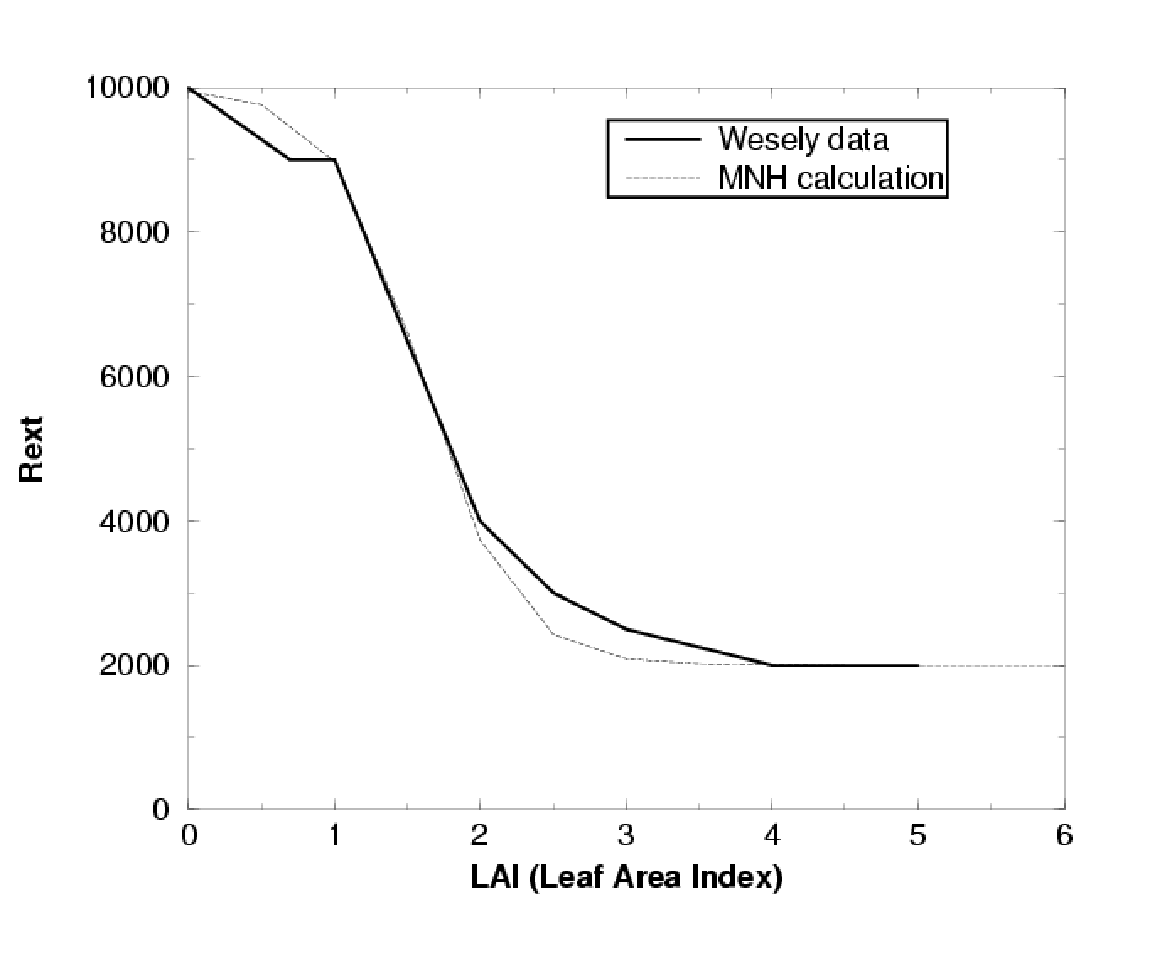
\psfig{file=\EPSDIR/rext_lai.pdf,width=0.5\textwidth}}
\label{lai_rext}
\caption{\sl{$\bf{R_{ext}}$ fonction of $\bf{LAI}$ (from Wesely table)}}
\end{figure}

\begin{table}
\begin{center}
\begin{tabular}{lllllllllll}
\hline
1&2&3&4&5&6&7&8&9&10&11 \\ \hline
\multicolumn{11}{l}{Midsummer with lush vegetation}\\
9999 & 2000& 2000&   2000   & 2000  & 2000  & 9999 & 9999 & 2500 & 2000 & 4000
\\
\multicolumn{11}{l}{Autumn with unharvested cropland}\\
9999 & 9000& 9000&   9000   & 4000  & 8000  & 9999 & 9999 & 9000 & 9000 & 9000
\\
\multicolumn{11}{l}{Late autumn after frost, no snow}\\
9999 & 9999 & 9000&   9000   & 4000  & 8000  & 9999 & 9999 & 9000 & 9000 & 9000
\\
\multicolumn{11}{l}{Winter}\\
9999 & 9999 & 9999 & 9999 & 6000  & 9000  & 9999 & 9999 & 9000 & 9000 & 9000
\\
\multicolumn{11}{l}{Spring}\\
9999 & 4000& 4000&   4000   & 2000  & 3000  & 9999& 9999&  4000 & 4000 & 8000
\\ \hline
\end{tabular}
\caption { \sl~{Input resistances for calculation of external leaf resistance
(Wesely,1989) : (1)urban land, (2)agricultural land, (3)range land,
(4)deciduous forest, (5)coniferous forest, (6)mixed forest
including wetland, (7)water, (8)barren land, mostly desert,
(9)nonforested wetland, (10)mixed agricultural and range land,
(11)rocky-open areas with low-growing shrubs}} 
\label{resdebase}

\end{center}
\end{table}

In case of dew or rain, and according to the same author and
Walmsley and Wesely (1996)\nocite{Walmsley1996}, the equation should be replaced by :
\[R_{ext.x.wet}=[1/(3R_{ext.x.dry})+(10^{-7}H^*+f_0/R_{extOzone}]^{-1}\]
with

\begin{itemize}
 
\item { Rain : \[ R_{extOzone} = (1/(3R_{ext})+1/1000 )^{-1}\]  }
 
\item { Dew : \[ R_{extOzone} = (1/(3R_{ext})+1/3000 )^{-1}\]  }
\end{itemize}
 
To apply the same comput for each species we approximate in case of
wet soil these formulas by 
using $R_{extOzone}$ as 3000 s/m .

These formulas should be corrected when surface
temperature decreases below -2$^o$C by adding the value
$1000 \exp (-T-4)$, in order to take into acccount the lesser uptake
by surfaces 
when cold.
%----------------GG6---------------------
\subsubsection*{In-canopy transport $R_{inc}$}

Deposition to soils under vegetation can be relatively important. 
Meyers and Baldocchi (1988) found that 20\% - 30\% of SO$_2$ was deposited 
in summer to the soil under a deciduous forest.
This transport is due to large-scale intermittent eddies through the
vegetation. 
The corresponding resistance has been parametrized by Erisman and Baldocchi (1994)
using data of VanPul and Jacobs (1994)\nocite{VanPul1994}
as :
\[ R_{inc}=\frac{b\; {\bf LAI}\; h}{\bf{u^*}}\]        %LAI_PATCH
$b$ is an empirical constant estimated at 14 $m^{-1}$. $\bf LAI=
LAI\_patch$ is the  
leaf area index given by patches computed in the GROUND\_PARAMn files
and $\bf h$ is the 
vegetation height which can be calculated as four times the 
vegetation roughness length
(formula of Kondo and Yamazawa (1986)\nocite{Kondo1986}, assuming a dense vegetation canopy
with similar height).

\medskip
%----------------GG7---------------------
\subsubsection*{Soil resitances for surfaces with no vegetation and those
under vegetation}
Table \ref{rsol} presents a review of soil resistances for SO$_2$ and O$_3$
for clay, sand, snow and it is completed
with table \ref{rcsoil}, Wesely value for all other vegetation types, 
town and rock.\\
For other gases, the resistance can be computed following Wesely (1989) :
\[ R_{soilx} = (\frac{H^*}{10^5 R_{soilSO_2}}+ \frac{f_0}{R_{soilO_3}})^{-1} \]
According to the same author, this formula should be corrected when surface
temperature decreases below -2$^o$C by adding the value :
\[R_{soilx} =  R_{soilx} + 1000 \exp (-T-4) \]
For no vegetation cover soil surface composition
(sand, clay) is considered. If it is 
covered by snow, this formlation will be update by using table \ref{rsol}. 
\[ R_{sandx} = (\frac{H^*}{10^5 R_{sandSO_2}}+ \frac{f_0}{R_{sandO_3}})^{-1} \]
\[ R_{clayx} = (\frac{H^*}{10^5 R_{claySO_2}}+ \frac{f_0}{R_{clayO_3}})^{-1} \]
\[ R_{snowx} = (\frac{H^*}{10^5 R_{snowSO_2}}+ \frac{f_0}{R_{snowO_3}})^{-1} \]
In this context $R_{no.x}$ for bare ground (no veg.) without snow is
the weighted average of $R_{sandx}$ and $R_{clayx}$ as: 
$$ R_{no.x} = ( \frac{\alpha_{sand}}{R_{sandx}} +
                \frac{\alpha_{clay}}{R_{clayx}} )^{-1} $$
with\\
$\alpha_{sand}$ : percentage of sand in the ground \\
$\alpha_{clay}$ : percentage of clay in the ground \\
For all the other type of soil, resistance is calculated with table
\ref{rcsoil} as :
\begin{eqnarray*} 
R_{rockx} & = & (\frac{H^*}{10^5 R_{rockSO_2}}+
        \frac{f_0}{R_{rockO_3}})^{-1}  \\
R_{townx} & = & (\frac{H^*}{10^5 R_{townSO_2}}+
        \frac{f_0}{R_{townO_3}})^{-1} \\
R_{c3x} & = & (\frac{H^*}{10^5 R_{c3SO_2}}+ \frac{f_0}{R_{c3O_3}})^{-1} \\
R_{c4x} & = & (\frac{H^*}{10^5 R_{c4SO_2}}+ \frac{f_0}{R_{c4O_3}})^{-1} \\
R_{treex} & = & (\frac{H^*}{10^5 R_{treeSO_2}}+
        \frac{f_0}{R_{treeO_3}})^{-1} \\
R_{grassx} & = & (\frac{H^*}{10^5 R_{grassSO_2}}+
        \frac{f_0}{R_{grassO_3}})^{-1} \\
R_{irrx} & = & (\frac{H^*}{10^5 R_{irrSO_2}}+
        \frac{f_0}{R_{irrO_3}})^{-1} \\
R_{parkx} & = & (\frac{H^*}{10^5 R_{parkSO_2}}+
        \frac{f_0}{R_{parkO_3}})^{-1} \\
\end{eqnarray*}

\begin{table}
\begin{center}
\begin{tabular}{lll}\hline
Type of soil & SO$_2$                    & O$_3$  \\ \hline
snow           & 540 at T $ < $-1$^o$C      & 2000   \\ 
               & 70(2-T) at -1 $<$ T $<$ 1 &        \\ 
sand           & 1000                      & 200    \\ 
clay           & 1000                      & 100    \\  \hline
\end{tabular}
\caption{\sl ~{Soil resistance}}
\label{rsol}
\end{center}
\end{table}

\begin{table}
\begin{center}
\begin{tabular}{llllllllll}\hline
\multicolumn{10}{l}{MNH cover type}\\
 c3 & c4 & tree & grass & no & rock & snow/ice & irr & park & town \\ 
\hline
\multicolumn{10}{l}{Soil resistance for SO$_2$}\\
150 & 150 & 500 & 350 & 1000 & 400 & no data & 0 & 100 & 400 \\
\hline
\multicolumn{10}{l}{Soil resistance for O$_3$}\\
150 & 150 & 200 & 200 & 400 & 200 & no data & 1000 & 700 & 300 \\
\hline  
\end{tabular}
\caption{\sl ~{Soil resistance for MNH-C decomposition from Wesely
table (quasi constant during the year). Values for ``snow/ice'' and
``no'' (no veg.) are not used see table \ref{rsol}.}} 
\label{rcsoil}
\end{center}
\end{table}

\subsubsection*{Surfaces resistances for sea and water}
For deposition over water surface bodies, the surface resistance can
be calculated from the expression recommended by Sehmel (1980) that
incorporates wind speed and 
and air/water partitioning coefficient, rather than from Wesely's
tabulated values for water bodies. The surface resistance over water
is: 

\[R_{waterx} = \frac{2,54 . 10^{-4}}{H^* \bf{T_{water}} u_*}  = Rc_{waterx}\] 
\[R_{seax} = \frac{2,54 . 10^{-4}}{H^* \bf{T_{sea}} u_*}  = Rc_{seax}\]
 
\subsection{Dry deposition velocity formulation}

\subsubsection*{Artificial land resistance}
$$ Rglobal^{town} = Ra^{town} + Rb^{town} + Rc^{town} $$
\subsubsection*{Sea and water resistance}
$$Rglobal^{water} = Ra^{water} + Rb^{water} + Rc^{water}$$\\
$$Rglobal^{sea} = Ra^{sea} + Rb^{sea} + Rc^{sea}$$
\subsubsection*{Nature final resistance}
$$ Rglobal^{nature} = \sum_{i=1}^{nvegtype} {\left(
\frac{\alpha_i}{Ra^{j_{patch}} + Rb^{j_{patch}} + Rc^{i} }\right)^{-1}} $$
with\\
$i \stackrel{f}{\longmapsto} f(i) = j_{patch}$ like
 $i \in [1,nvegtype]$, $f(i)=j_{patch} \in [1,npatch\leq nvegtype]$ \\
and 
 $ \alpha_i $ fraction of cover type (9 types)

\subsubsection*{Dry deposition velocity}

Final dry deposition formulation:
$$
v_{dry deposition} = \frac{\alpha_{water}}{Rglobal^{water}} +
\frac{\alpha_{sea}}{Rglobal^{sea}} +
\frac{\alpha_{townmax}}{Rglobal^{town}} +
\frac{\alpha_{nature}}{Rglobal^{nature}}
$$
where\\ 
\begin{tabbing}
$\alpha_{townmax}$ \=: fraction of town increased \kill
$\alpha_{water}$ \> : fraction of water \\
$\alpha_{sea}$ \> : fraction of sea \\
$\alpha_{townmax}$ \> : fraction of town increased \\
$\alpha_{sea}$ \> : fraction of nature 
\end{tabbing}
Fraction of town has to be increased in order to take account of the non
negligible dry deposition on vertical surfaces in artificial
area. The increase is done as follows :\\
$\alpha_{townmax} = \alpha_{town} (1+2 \frac{H}{L} \, \alpha_{bld})$
with : \\
$\alpha_{town}$ horizontal fraction of town \\
$H$ building height \\
$L$ building caracteristic width \\
$\alpha_{bld}$ fraction of buildings in artificial areas (only)
\begin{figure}[hbp]
\begin{center}
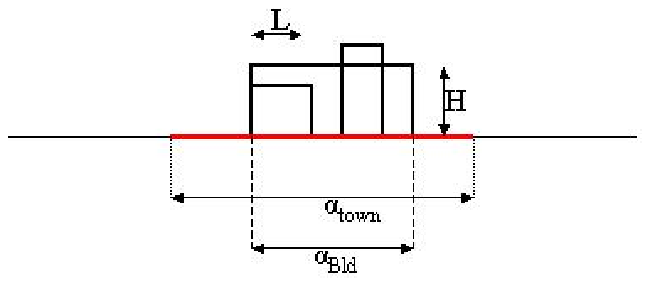
\includegraphics[width=15cm,height=5cm]{\EPSDIR/xbldmax.pdf}
\end{center}
\label{bld}
\caption{\sl{town parameters in MNH (modd\_gr\_field) to increase
fraction of town}} 
\end{figure}

\section{Dry deposition of aerosols}
\subsection*{Brownian diffusivity and sedimentation velocity}

Dry deposition and sedimentation of aerosols are driven by the Brownian 
diffusivity:
\begin{equation}
D_p = \left(\frac{k T}{6 \pi \nu \rho_{air} r_p} \right) C_c
\label{diff_bro}
\end{equation}
and by  the gravitational velocity:
\begin{equation}
V_g = \left(\frac{2 g}{9 \nu}\left(\frac{\rho_{p,i}}{\rho_{air}}\right) r_p^2 
\right) C_c
\label{vitesse_grav}
\end{equation}
where $k$ is the Bolzmann constant, $T$ the ambient temperature, $\nu$ the air 
kinematic velocity, $\rho_{air}$ the air density, $g$ the gravitational 
acceleration, $\rho_{p,i}$ the aerosol density of mode $i$, and $C_c = 1 + 
1.246\frac{\lambda_{air}}{r_p}$ the gliding coefficient. 
These expressions need to be averaged on the $k^{th}$ moment and mode $i$ as:
\begin{equation}
\hat{X} = \frac{1}{M_{k,i}} \int_{-\infty}^{\infty} X r^k_p n_i(\ln r_p)d(\ln r_p)
\label{moyenne}
\end{equation}
where $X$ represents either $D_p$ or $v_g$.
After integration, we obtain for  Brownian diffusivity:
\begin{equation}
\hat{D}_{p_{k,i}} = \tilde{D}_{p_{g,i}}\left[\exp\left(\frac{-2k+1}{2} 
\ln^2\sigma_{g,i} \right) + 1.246 Kn_g 
\exp \left(\frac{-4k+4}{2} \ln^2\sigma_{g,i}\right) \right]
\label{diff_brow}
\end{equation}
with $\tilde{D}_{p_{g,i}} = \left(\frac{kT}{6 \pi \nu \rho_{air} R_{g,i}} 
\right)$

and for gravitational velocity: 
\begin{equation}
\hat{Vg}_{p_{k,i}} = \tilde{Vg}_{p_{g,i}}\left[\exp\left(\frac{4k+4}{2} 
\ln^2\sigma_{g,i} \right) + 1.246 Kn_g \exp \left(\frac{2k+4}{2} 
\ln^2\sigma_{g,i}\right) \right]
%\label{gravi_vel}
\end{equation}
with $\tilde{Vg}_{p_{g,i}} = \left(\frac{2g \rho_{p,i}}{9 \nu \rho_{air}} 
R_{g,i}^2 \right)$

\subsection*{Dry deposition}
According to Seinfeld and Pandis (1997)\nocite{seinfeld1997} and using the resistance concept of 
Wesely (1989), aerosol dry deposition
velocity for the $k^{th}$ moment and mode $i$ is:
\begin{equation}
\hat{v}_{d_{k,i}} = ( r_a + \hat{r}_{d_{k,i}} + r_a  \hat{r}_{d_{k,i}} 
\hat{Vg}_{p_{k,i}})^{-1} + \hat{Vg}_{p_{k,i}}
%\label{gravi_vel}
\end{equation}
where surface resistance $\hat{r}_{d_{k,i}}$ is given by
\begin{equation}
\hat{r}_{d_{k,i}} = \left[(\hat{Sc}_{k,i}^{-2/3} + 10^{-3/\hat{St}_{k,i}}) 
\left(1+ 0.24 \frac{w_*^2}{u_*^2} \right) u_* \right]^{-1}
\label{surfres}
\end{equation}
Schmidt and Stokes number are respectively equal to $\hat{Sc}_{k,i} = \nu / 
\hat{D}_{p_{k,i}}$ and
$\hat{St}_{k,i}= (u_*^2/g\nu)\hat{v}_{d_{k,i}}$.
One can observe that the friction velocity $u_*$ and the convective velocity 
$w_*$ depend on meteorological
and surface conditions. 
\section{Biogenic VOC fluxes}
Biogenic fluxes are parameterize on-line in the surfex code.
For a model grid-cell, biogenic fluxes of isoprene and monoterpenes are calculated according to the classical Guenther’s approach (Guenther \etal (1994,~1995)\nocite{Guenther1994,Guenther1995}), using the general formulation :

\begin{equation}
F^{cell}_x =  \sum_{N} \nu_n  X . EP_{x,n} X . ECF_{x,n}
\label{biogenic}
\end{equation}
Where Fxcell (in µg.m-2.h-1) is the grid-cell averaged biogenic fluxes in which x refers either to isoprene or monoterpenes. $\nu_n$ represents the surface fractions occupied by N sub-grid emitting ecosystems (forests, shrublands, crops, etc). The related emission potential, $EP_{x,n}$, (in $\mu g.m^{-2}.h^{-1}$), accounts for the emission capacity of the underlying nth ecosystem under fixed climatic conditions. According to Guenther’s approach, EPiso is standardized to a surface vegetation temperature Ts of 303 K and a photosynthetically active radiation (par) of 1000 $\mu E.m^{-2}.s^{-1} $, whereas EPmono is generally standardized only for Ts =303 K. The temporal evolution of fluxes is given by environmental correction factors ECFx,n calculated from the canopy micro-climates of the N underlying ecosystems. This formulation assumes a simple homogeneous vertical leaf distribution in ecosystem canopies.
Over France, emission potential have been pre calculated by GIS treatment of land cover data base (Corine Land Cover), forest composition data for the main tree species (Inventaire forestier national) and species emission factors collected in the literature. The resulting emission potential maps are given at a resolution of 2km and are then interpolated on the MNH grid (during the prepPGD).
The environmental correction factor, which accounts for radiation and vegetation temperature variation effects on emissions is calculated using the surface energy budget (calculated by ISBA) and a simple in canopy radiation transfer scheme (similar as ISBA-Ags) for each of the ecosystem (Forest, shrublands, etc) contained in the model grid cells (cf PATCH approach). More details on the method can be found in Solmon \etal (2004)\nocite{Solmon2004}. 

%====================
\bibliography{surfex_scidoc}
%====================
